% last updated in April 2002 by Antje Endemann
% Based on CVPR 07 and LNCS, with modifications by DAF, AZ and elle, 2008 and AA, 2010, and CC, 2011

\documentclass[runningheads]{llncs}
\usepackage{graphicx}
\usepackage{amsmath,amssymb} % define this before the line numbering.
\usepackage{ruler}
\usepackage{color}
\usepackage[width=122mm,left=12mm,paperwidth=146mm,height=193mm,top=12mm,paperheight=217mm]{geometry}
\begin{document}
% \renewcommand\thelinenumber{\color[rgb]{0.2,0.5,0.8}\normalfont\sffamily\scriptsize\arabic{linenumber}\color[rgb]{0,0,0}}
% \renewcommand\makeLineNumber {\hss\thelinenumber\ \hspace{6mm} \rlap{\hskip\textwidth\ \hspace{6.5mm}\thelinenumber}}
% \linenumbers
\pagestyle{headings}
\mainmatter
\def\ECCV12SubNumber{***}  % Insert your submission number here

\title{Author Guidelines for ECCV Workshop Submission} % Replace with your title

\titlerunning{ECCV-12 submission ID \ECCV12SubNumber}

\authorrunning{ECCV-12 submission ID \ECCV12SubNumber}

\author{Anonymous ECCV submission}
\institute{Paper ID \ECCV12SubNumber}


\maketitle

\begin{abstract}
The abstract should summarize the contents of the paper and should
contain at least 70 and at most 300 words. It should be set in 9-point
font size and should be inset 1.0~cm from the right and left margins.
\dots
\end{abstract}


\section{Introduction}


Please follow the steps outlined below when submitting your manuscript.

%-------------------------------------------------------------------------

\subsection{Language}

All manuscripts must be in English.

\subsection{Paper length}
The basic length is 10 pages. Overlength papers will
simply not be reviewed. This includes papers where the margins and
formatting are deemed to have been significantly altered from those
laid down by this style guide.  The reason such papers will not be
reviewed is that there is no provision for supervised revisions of
manuscripts.

\subsection{Dual submission}

By submitting a manuscript to ECCV Workshops, the author(s) assert 
that it has not been previously published in substantially similar form. 
Furthermore, no paper which contains signi�cant overlap with the 
contributions of this paper either has been or will be submitted during 
the ECCV 2012 review period to either a journal or a conference. 
If there are any papers that may appear to the reviewers to violate this 
condition, then it is your responsibility to (1) cite these papers 
(preserving anonymity  as described in section 2 of this example paper, 
(2) argue in the body of your paper why your ECCV Workshop paper is 
nontrivially di?erent from these concurrent submissions, and (3) include 
anonymized versions of those papers in the supplemental material.

\subsection{Supplemental Material}

Authors may optionally upload supplemental material. Typically, this 
material might include videos of results that cannot be included in 
the main paper, anonymized related submissions to other conferences 
and journals, and appendices or technical reports containing extended 
proofs and mathematical derivations that are not essential for understanding 
of the paper. Note that the contents of the supplemental material should be 
referred to appropriately in the paper and that reviewers are not obliged to look at it. 
All supplemental material must be zipped or tarred into a single �le. 
There is a 50MB limit on the size of this �le. The deadline for supplemental 
material is �ve days after the main paper deadline. 

%-------------------------------------------------------------------------
\subsection{Line numbering}

All lines should be numbered, as in this example document.  This makes
reviewing more efficient, because reviewers can refer to a line on a
page.  If you are preparing a document using a non-\LaTeX\
document preparation system, please arrange for an equivalent line numbering.

\subsection{Mathematics}

Please number all of your sections and displayed equations.  Again,
this makes reviewing more efficient, because reviewers can refer to a
line on a page.  Also, it is important for readers to be able to refer
to any particular equation. Some authors might benefit from
reading Mermin's description of how to write mathematics:
\url{http://www.cvpr.org/doc/mermin.pdf}.


\section{Blind review}
\label{sec:blind}

Many authors misunderstand the concept of anonymizing for blind
review.  Blind review does not mean that one must remove
citations to one's own work---in fact it is often impossible to
review a paper unless the previous citations are known and
available.

Blind review means that you do not use the words ``my'' or ``our''
when citing previous work.  That is all.  
If you are making a submission to another conference at the same
time, which covers similar or overlapping material, you may need
to refer to that submission in order to explain the differences,
just as you would if you had previously published related work. 



\section{Manuscript Preparation}
For your manuscript preparation, you can refer to the edited version of 
Springer LNCS instructions adapted for ECCV 2012 

You are strongly encouraged to use \LaTeX2$_\varepsilon$ for the
preparation of your
camera-ready manuscript together with the corresponding Springer
class file \verb+llncs.cls+.

We would like to stress that the class/style files and the template
should not be manipulated and that the guidelines regarding font sizes
and format should be adhered to. This is to ensure that the end product
is as homogeneous as possible.

\subsection{Printing Area}
The printing area is $122  \; \mbox{mm} \times 193 \;
\mbox{mm}$.
The text should be justified to occupy the full line width,
so that the right margin is not ragged, with words hyphenated as
appropriate. Please fill pages so that the length of the text
is no less than 180~mm.

\subsection{Layout, Typeface, Font Sizes, and Numbering}
Use 10-point type for the name(s) of the author(s) and 9-point type for
the address(es) and the abstract. For the main text, please use 10-point
type and single-line spacing.
We recommend using Computer Modern Roman (CM) fonts, Times, or one
of the similar typefaces widely used in photo-typesetting.
(In these typefaces the letters have serifs, i.e., short endstrokes at
the head and the foot of letters.)
Italic type may be used to emphasize words in running text. Bold
type and underlining should be avoided.
With these sizes, the interline distance should be set so that some 45
lines occur on a full-text page.

\subsubsection{Headings.}

Headings should be capitalized
(i.e., nouns, verbs, and all other words
except articles, prepositions, and conjunctions should be set with an
initial capital) and should,
with the exception of the title, be aligned to the left.
Words joined by a hyphen are subject to a special rule. If the first
word can stand alone, the second word should be capitalized.
The font sizes
are given in Table~\ref{table:headings}.
\setlength{\tabcolsep}{4pt}
\begin{table}
\begin{center}
\caption{Font sizes of headings. Table captions should always be
positioned {\it above} the tables. The final sentence of a table
caption should end without a full stop}
\label{table:headings}
\begin{tabular}{lll}
\hline\noalign{\smallskip}
Heading level & Example & Font size and style\\
\noalign{\smallskip}
\hline
\noalign{\smallskip}
Title (centered)  & {\Large \bf Lecture Notes \dots} & 14 point, bold\\
1st-level heading & {\large \bf 1 Introduction} & 12 point, bold\\
2nd-level heading & {\bf 2.1 Printing Area} & 10 point, bold\\
3rd-level heading & {\bf Headings.} Text follows \dots & 10 point, bold
\\
4th-level heading & {\it Remark.} Text follows \dots & 10 point,
italic\\
\hline
\end{tabular}
\end{center}
\end{table}
\setlength{\tabcolsep}{1.4pt}

Here are
some examples of headings: ``Criteria to Disprove Context-Freeness of
Collage Languages'', ``On Correcting the Intrusion of Tracing
Non-deterministic Programs by Software'', ``A User-Friendly and
Extendable Data Distribution System'', ``Multi-flip Networks:
Parallelizing GenSAT'', ``Self-determinations of Man''.

\subsubsection{Lemmas, Propositions, and Theorems.}

The numbers accorded to lemmas, propositions, and theorems etc. should
appear in consecutive order, starting with the number 1, and not, for
example, with the number 11.

\subsection{Figures and Photographs}
\label{sect:figures}

Please produce your figures electronically and integrate
them into your text file. For \LaTeX\ users we recommend using package
\verb+graphicx+ or the style files \verb+psfig+ or \verb+epsf+.

Check that in line drawings, lines are not
interrupted and have constant width. Grids and details within the
figures must be clearly readable and may not be written one on top of
the other. Line drawings should have a resolution of at least 800 dpi
(preferably 1200 dpi).
For digital halftones 300 dpi is usually sufficient.
The lettering in figures should have a height of 2~mm (10-point type).
Figures should be scaled up or down accordingly.
Please do not use any absolute coordinates in figures.

Figures should be numbered and should have a caption which should
always be positioned {\it under} the figures, in contrast to the caption
belonging to a table, which should always appear {\it above} the table.
Please center the captions between the margins and set them in
9-point type
(Fig.~\ref{fig:example} shows an example).
The distance between text and figure should be about 8~mm, the
distance between figure and caption about 5~mm.
\begin{figure}
\centering
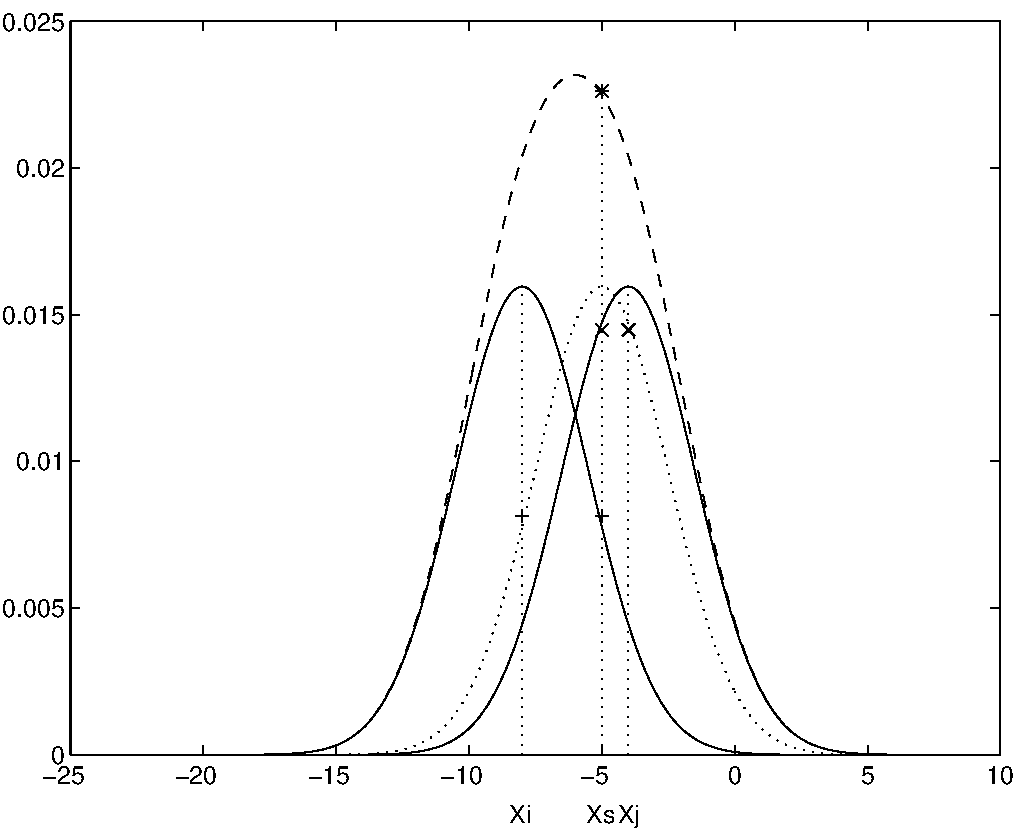
\includegraphics[height=7.2cm]{eijkel2}
\caption{One kernel at $x_s$ ({\it dotted kernel}) or two kernels at
$x_i$ and $x_j$ ({\it left and right}) lead to the same summed estimate
at $x_s$. This shows a figure consisting of different types of
lines. Elements of the figure described in the caption should be set in
italics,
in parentheses, as shown in this sample caption. The last
sentence of a figure caption should generally end without a full stop}
\label{fig:example}
\end{figure}

If possible (e.g. if you use \LaTeX) please define figures as floating
objects. \LaTeX\ users, please avoid using the location
parameter ``h'' for ``here''. If you have to insert a pagebreak before a
figure, please ensure that the previous page is completely filled.


\subsection{Formulas}

Displayed equations or formulas are centered and set on a separate
line (with an extra line or halfline space above and below). Displayed
expressions should be numbered for reference. The numbers should be
consecutive within the contribution,
with numbers enclosed in parentheses and set on the right margin.
For example,
\begin{align}
  \psi (u) & = \int_{0}^{T} \left[\frac{1}{2}
  \left(\Lambda_{0}^{-1} u,u\right) + N^{\ast} (-u)\right] dt \; \\
& = 0 ?
\end{align}

Please punctuate a displayed equation in the same way as ordinary
text but with a small space before the end punctuation.

\subsection{Program Code}

Program listings or program commands in the text are normally set in
typewriter font, e.g., CMTT10 or Courier.

\medskip

\noindent
{\it Example of a Computer Program}
\begin{verbatim}
program Inflation (Output)
  {Assuming annual inflation rates of 7%, 8%, and 10%,...
   years};
   const
     MaxYears = 10;
   var
     Year: 0..MaxYears;
     Factor1, Factor2, Factor3: Real;
   begin
     Year := 0;
     Factor1 := 1.0; Factor2 := 1.0; Factor3 := 1.0;
     WriteLn('Year  7% 8% 10%'); WriteLn;
     repeat
       Year := Year + 1;
       Factor1 := Factor1 * 1.07;
       Factor2 := Factor2 * 1.08;
       Factor3 := Factor3 * 1.10;
       WriteLn(Year:5,Factor1:7:3,Factor2:7:3,Factor3:7:3)
     until Year = MaxYears
end.
\end{verbatim}
%
\noindent
{\small (Example from Jensen K., Wirth N. (1991) Pascal user manual and
report. Springer, New York)}


\subsection{Footnotes}

The superscript numeral used to refer to a footnote appears in the text
either directly after the word to be discussed or -- in relation to a
phrase or a sentence -- following the punctuation sign (comma,
semicolon, or full stop). Footnotes should appear at the bottom of
the
normal text area, with a line of about 2~cm in \TeX\ and about 5~cm in
Word set
immediately above them.\footnote{The footnote numeral is set flush left
and the text follows with the usual word spacing. Second and subsequent
lines are indented. Footnotes should end with a full stop.}

\subsection{Citations}

The list of references is headed ``References" and is not assigned a
number
in the decimal system of headings. The list should be set in small print
and placed at the end of your contribution, in front of the appendix,
if one exists.
Please do not insert a pagebreak before the list of references if the
page is not completely filled.
An example is given at the
end of this information sheet. For citations in the text please use
square brackets and consecutive numbers: \cite{Alpher02},
\cite{Alpher03}, \cite{Alpher04} \dots


\bibliographystyle{splncs}
\bibliography{egbib}

\clearpage\mbox{}Page \thepage\ of the manuscript.
\clearpage\mbox{}Page \thepage\ of the manuscript.
\clearpage\mbox{}Page \thepage\ of the manuscript.
\clearpage\mbox{}Page \thepage\ of the manuscript.

This is the last page of the manuscript.
\par\vfill\par
Now we have reached the maximum size of the ECCV 2012 submission.
\end{document}
